\chapter{ارزیابی روش پیشنهادی}
\section{مقدمه}

در این کار سعی بر این داشته‌ایم تا به کمک روش‌های یادگیری ژرف در راستای شناسایی چهره در ویدیوهای بدون محدودیت قدمی برداریم و در این حوزه عملکرد هوش مصنوعی و یادگیری ژرف را بهبود دهیم. بنابراین با تحقیق و آزمایش روشی برای دسته بندی دقیق تر چهره افراد در تصاویر ویدیویی پیشنهاد داده‌ایم که شرح آن در فصل قبل انجام شد و نوبت آن است که الگوریتم پیشنهادی را ارزیابی کرده و با بیان نتایج به مقایسه با کارهای دیگر می‌پردازیم.

\section{معیار ارزیابی}
یکی از معیارهایی که بسیار در زمینه‌های تحقیقاتی و مسائل دسته بندی حائز اهمیت است، معیار دقت می‌باشد. در این کار ما با تصاویر چهره دارای هویت های مختلف سر و کار داریم. بنابراین معیار دقت در این کار به معنی درصد نمونه‌هایی است که هویت آن‌ها به درستی تشخیص داده شده است. فرمول این معیار در رابطه \ref{eq5-1} بیان شده است.

\begin{equation}\label{eq5-1}
Accuracy= \frac{TP+TN}{P+N}
\end{equation}

\noindent
که در آن مثبت‌های صحیح \LTRfootnote{True Positive} یا $TP$ تعداد نمونه‌هایی است که به درستی تشخیص داده شده‌اند. منفی‌های صحیح \LTRfootnote{True Negative} یا $TN$ تعداد نمونه‌هایی است که به درستی تشخیص داده نشده‌اند. مقدار $P$ تعداد کل تصاویر مثبت و $N$ تعداد کل تصاویر منفی را نشان می‌دهد.

\noindent
همانطور که می‌دانیم، به طور معمول معماری های شبکه عصبی عمیق تر، دارای دقت بالاتر و همچنین زمان پردازش بیشتری می‌باشند. از طرفی هرچه معماری شبکه عصبی، سبک تر و تعداد پارامترهای آن کمتر باشد، می‌توان انتظار داشت که سرعت بالاتری در زمان اجرا داشته باشد، اما دقت آن با کاهش همراه است. بر همین اساس در مقابل معیار دقت، معیار دیگری به نام تراکم دقت یا چگالی دقت وجود دارد که از تقسیم مقدار دقت بر تعداد پارامترهای معماری شبکه بدست می‌آید و می‌تواند معیار خوبی برای ارزیابی دقت معماری‌های مختلف نسبت به سرعت اجرای آن‌ها باشد.
‌\begin{equation}\label{eq5-2}
Accuracy Density = \frac{Accuracy}{Mparams}
\end{equation}

\noindent
که در آن \lr{Mparams} تعداد پارامترهای شبکه بر حسب میلیون می‌باشد.

\section{مجموعه داده}
در زمینه تشخیص چهره، مجموعه داده‌های بسیار زیادی وجود دارند. تعدادی از این مجموعه داده‌ها، حاوی تصاویر چهره در محیط‌های آزمایشگاهی و کنترل شده می‌باشند که در بحث ما گنجانده نمی‌شوند. با رشد الگوریتم های یادگیری عمیق و بدست آمدن نتایح مناسب در زمینه تشخیص چهره، مجموعه داده‌های جدیدتری منتشر شدند که دارای تصاویر چهره در محیط‌های بدون محدودیت هستند. بیشتر مقالات معتبری که در فصل‌های قبل به آن‌ها اشاره شد، برخی از این مجموعه داده‌ها را برای آموزش و برخی را برای آزمون استفاده کرده‌اند. ما نیز مجموعه داده‌ها را بر همین اساس دسته بندی کرده‌ایم که به شرح آن‌ها می‌پردازیم.

\subsection{مجموعه داده‌های آموزش}
ما ترکیبی از سه مجموعه داده مشهور در زمینه تشخیص چهره را برای آموزش استفاده کردیم که عبارت‌اند از:
\subsubsection{مجموعه داده \lr{CASIA Web-Face}}
مجموعه داده CASIA Web-Face که شامل ۴۹۴۴۱۴ تصویر چهره متفاوت از ۱۰۵۷۵ فرد است، بدون برچسب اشتباه است. این مجموعه داده در مسائل تایید چهره و تشخیص چهره کاربرد دارد. \cite{CASIA_dataset}

\subsubsection{مجموعه داده \lr{MS-Celeb-1M}}
مجموعه داده MS-Celeb-1M \LTRfootnote{Microsoft celebrities} که به مراتب مجموعه داده بزرگتری محسوب می شود، شامل بیش از ۸ میلیون تصویر چهره متفاوت از 100 هزار فرد است. برخلاف مجموعه داده \lr{CASIA Web-Face}، این مجموعه‌داده با نویز و برچسب اشتباه همراه است. این مجموعه داده را شرکت مایکروسافت ایجاد کرده است. \cite{MS_Celeb_dataset}

\subsubsection{مجموعه داده \lr{VGGFace2}}
محققان دانشگاه آکسفورد نسخه 2 مجموعه‌داده‌ \lr{VGGFace} را با 3.31 میلیون تصویر از 9131 فرد مختلف ارائه کردند. این تصاویر با کمک جست‌و‌جوی تصویر گوگل جمع‌آوری ‌شده و شامل تغییرات مختلف برای هر فرد نظیر سن، جهت، نور و ... هستند. این مجموعه‌داده شامل افراد مختلفی نظیر سیاست‌مداران، ورزشکاران، بازیگران و ... است و به‌طور تقریبی از هر فرد 362 تصویر مختلف موجود است. \cite{VGGFace2_dataset}

\subsection{مجموعه داده‌های آزمون}
ما ترکیبی از سه مجموعه داده مشهور در زمینه تشخیص چهره را برای آموزش استفاده کردیم که عبارت‌اند از:

\subsubsection{مجموعه داده \lr{LFW}}
مجموعه داده LFW \LTRfootnote{Labeled Faces in the Wild} که شامل 13233 تصویر چهره متفاوت از ۵۷۴۹ فرد مختلف است، از اولین مجموعه داده های منتشر شده برای مسائل تشخیص چهره بدون محدودیت می باشد. \cite{LFW_dataset}

\subsubsection{مجموعه داده \lr{PubFig}}
مجموعه داده PubFig \LTRfootnote{Public Figures} که شامل ۵۸۷۹۷ تصویر چهره متفاوت از ۲۰۰ فرد است، از اینترنت جمع آوری شده است. این تصاویر شامل تغییرات مختلف مانند جهت، نور، انسداد و ... هستند. \cite{PubFig_dataset}

\subsubsection{مجموعه داده \lr{YouTube Faces}}
این مجموعه داده برای استفاده در کارهای تشخیص چهره در تصاویر ویدیویی ایجاد شده است. این مجموعه داده شامل ۳۴۲۵ ویدیو از ۱۵۹۵ فرد مختلف است و تمام ویدیوها از سایت یوتیوب دانلود شده اند. به طور میانگین 2.15 فیلم برای هر شخص در دسترس است. کوتاه ترین مدت ویدیو 48 فریم ، طولانی ترین ویدیو 6070 فریم و متوسط طول یک ویدیو 181.3 فریم است. \cite{VGGFace2_dataset}

\subsubsection{مجموعه داده \lr{CFP}}
مجموعه داده CFP \LTRfootnote{Celebrities in Frontal-Profile in the Wild} که شامل ۷۰۰۰ تصویر چهره متفاوت از ۵۰۰ فرد است، تصاویر افراد مشهور را در حالت های تمام رخ و نیم رخ جمع آوری کرده است. این مجموعه داده می‌تواند ابزار ارزیابی بسیار خوبی برای چالش زاویه چهره باشد. \cite{LFW_dataset}

\subsubsection{مجموعه داده \lr{CACD}}
مجموعه داده CACD \LTRfootnote{Cross-Age Celebrity Dataset} شامل 163446 تصویر از 2000 فرد مشهور است که از اینترنت جمع آوری شده است. تصاویر از موتورهای جستجو با استفاده از نام افراد مشهور و سال (2004-2013) به عنوان کلمات کلیدی جمع آوری شده است. بنابراین ، می توان با تفریق سال تولد افراد از سال عکس گرفته شده، به سادگی سن افراد در تصاویر را تخمین زد. این مجموعه داده می‌تواند ابزار ارزیابی بسیار خوبی برای چالش تغییرات سن باشد. \cite{CACD_dataset}

\subsubsection{مجموعه داده \lr{MegaFace}}
محققان دانشگاه واشنگتن مجموعه داده MegaFace \LTRfootnote{Million-Scale Face Recognition Dataset} عظیم را ارائه کرده اند که هم در مسائل تایید چهره و هم در مسائل تشخیص چهره کاربرد دارد. این مجموعه داده شامل یک زیر مجموعه آزمایش است که خود از دو مجموعه \lr{FaceScrub} شامل تصاویر افراد مشهور و \lr{FGNet} شامل تصاویر مخصوص چالش سن، تشکیل شده است. اگر الگوریتم مورد نظر بر روی مجموعه \lr{FGNet} دقت بالا بدست آورد، نشان دهنده قوت الگوریتم در تصاویر با تفاوت سن‌های بالا می‌باشد \cite{MegaFace_dataset}. اطلاعات تکمیلی درباره مجموعه داده‌های آزمایش را در جدول \ref{table5-1} مشاهده می‌نمایید.

\begin{table}[ht]
\label{table5-1}
\caption{مجموعه‌داده های ارزیابی رایج در زمینه بازشناسی چهره}
\begin{center}
\resizebox{\textwidth}{!}
{
\begin{tabular}{|c|c|c|c|}
\hline 
نام & تعداد تصاویر چهره & تعداد افراد & نوع کاربرد
\\
\hline 
\lr{LFW}
& 13233	 & ۵۷۴۹ & 	تشخیص چهره 
 \\
\hline
\lr{PubFig}
& ۵۸۷۹۷	 & ۲۰۰ & 	تشخیص چهره 
\\
\hline
\lr{YouTube Faces}
& ۳۴۲۵ ویدیو	 & ۱۵۹۵ & 	تشخیص چهره
\\
\hline 
\lr{CFP}
& ۷۰۰۰	 & ۵۰۰ & 	تشخیص چهره
\\
\hline
\lr{CACD}
& 163446	 & 2000 & 	تشخیص چهره
\\
\hline
\lr{MegaFace}
& ۱۰۰۰۰۰۰ + ۱۴۱۰۰۰ + ۹۷۵	 & ۶۹۰۰۰۰ + ۶۹۵ + ۸۲ & 	تشخیص چهره و تایید چهره
\\
\hline
\end{tabular}}
\end{center} 
\end{table} 

\section{پیکربندی الگوریتم}
به منظور آموزش شبکه‌، در هر دوره ۲۰٪ تعداد داد‌ه‌های آموزشی را به عناون داده‌های ارزیابی \LTRfootnote{Validation} در نظر می‌گیریم تا روند آموزش شبکه را بر اساس عامل‌های دیگر مورد بررسی قرار دهیم. همچنین در هر تکرار، اندازه دسته‌هایی که به شبکه برای آموزش داده می‌شود را برابر ۶۴ قرار دادیم. توصیه می‌شود این مقدار توانی از ۲ باشد که مقدار ۶۴ با تجربه و توجه به ظرفیت حافظه پردازنده گرافیکی بدست آمده است. از بهینه‌ساز Adam جهت آموزش استفاده کرده‌ایم. این بهینه‌ساز نیز نرخ آموزش را بر اساس خطا به صورت تطبیقی کم یا زیاد می‌کند. همچنین میانگین کاهش گرادیان‌های تکرارهای قبل را نگهداری می‌کند تا بر اساس آن‌ها جهت گرادیان تکرار جدید را محاسبه کند. برای تابع ضرر از معادله \ref{eq4-9} استفاده کرده‌‌ایم. این تابع میزان ضرر را به صورتی که در فصل قبل صحبت شد، محاسبه می‌کند.

\noindent
همچنین برای به دست آوردن بهترین نتیجه از آموزش، از روش ارزیابی تقاطعی استفاده کرده‌ایم. به این صورت که در هر مرتبه آموزش، تعداد داده‌های آموزش را به پنج دسته تقسیم می‌کنیم. چهار قسمت را برای آموزش و یک قسمت را برای ارزیابی در نظر می‌گیریم. به این ترتیب مدل شبکه را ۵ بار آموزش دادیم و بهترین نتیجه را برای آزمون بر روی مجموعه داده‌های آزمون انتخاب می‌کنیم.

\section{نتایج آزمون}
\subsection{دقت دسته بندی}
با توجه به پیکربندی بیان شده، مدل را آموزش داده‌ایم و به سراغ مجموعه داده‌های آزمون می‌رویم. مقدار دقت را طبق رابطه \ref{eq5-1} برای معماری‌های مرتبط و مشهور و همچنین روش پیشنهادی محاسبه کردیم. در جدول \ref{table5-2} نتایج حاصل از محاسبه دقت را در معماری‌های مختلف بر روی مجموعه داده‌های مشهور مشاهده می‌کنید.

\begin{table}[ht]
	\label{table5-2}
	\begin{center}
	\caption{دقت معماری‌های مختلف بر روی مجموعه‌داده‌های ارزیابی رایج در زمینه بازشناسی چهره}
	\resizebox{\textwidth}{!}
	{
		\begin{tabular}{|c|c|c|c|c|c|c|c|}
		\hline 
		\lr{Model} & \lr{Custom Dataset} & \lr{LFW} & \lr{AgeDB-30} & \lr{MegaFace}  & \lr{Mnist} & \lr{Cfar100} & \lr{ImageNet}
		\\
		\hline 
		\hline
		\lr{ArcFace} & \lr{99.70} & \lr{99.50} & \lr{95.91} & \lr{93.09} & & &  
		\\ 
		\hline
		\lr{MobileNetV3} & \lr{92.50} & \lr{98.10} & \lr{93.05} & \lr{90.59} & \lr{99.7} & \lr{80.01} & \lr{75.2}
		\\ 
		\hline
		\lr{SA-MobileNetV3} & \lr{99.80} & \lr{99.65} & \lr{96.02} & \lr{93.50} & \lr{99.9} & \lr{82.47} & \lr{79.8}
		\\
		\hline
		\end{tabular}
	}
	\end{center} 
\end{table} 

\noindent
ایده پایه در این پژوهش، طراحی یک عینک هوشمند با قابلیت شناسایی چهره برای افراد نابینا بود. در یک کاربرد واقعی، تعداد افراد آشنا برای یک شخص، محدود می‌باشد. بر همین اساس با در آزمونی دیگر با تعداد محدود داده‌های آموزشی، روش پیشنهادی را با روش دنگ و همکاران \cite{deng2019arcface} معروف به ArcFace مقایسه کردیم. در این ارزیابی که بر روی مجموعه داده LFW انجام شد، تعداد افراد آشنا را به ترتیب برابر با ۳۲، ۶۴، ۱۲۸ و ... در نظر گرفتیم و تعداد افراد ناشناس (افراد منفی) را برابر با تعداد افرادی که فقط یک تصویر از آن‌ها موجود می‌باشد، یعنی ۴۰۶۹ در نظر گرفتیم. نتایج ارزیابی در جدول \ref{table5-3} مشاهده می‌شود.

\begin{table}[ht]
	\label{table5-3}
	\begin{center}
		\caption{دقت بر روی مجموعه‌داده \lr{LFW} بر حسب تعداد متفاوت دسته‌ها}
		\resizebox{\textwidth}{!}
		{
			\begin{tabular}{|c|c|c|}
				\hline 
				\lr{Number of identites} & \lr{Accuracy (SA-MobileNetV3)} & \lr{Accuracy (Arcface-Mobilenet)}
				\\
				\hline 
				\hline
				\lr{32} & \lr{100} & \lr{100}
				\\ 
				\hline
				\lr{64} & \lr{100} & \lr{100}
				\\ 
				\hline
				\lr{128} & \lr{100} & \lr{99.97}
				\\ 
				\hline
				\lr{256} & \lr{99.95} & \lr{99.94}
				\\ 
				\hline
				\lr{512} & \lr{99.89} & \lr{99.89}
				\\ 
				\hline
				\lr{1024} & \lr{99.86} & \lr{99.86}
				\\ 
				\hline
				\lr{2048} & \lr{99.72} & \lr{99.69}
				\\ 
				\hline
				\lr{5016} & \lr{99.65} & \lr{99.50}
				\\ 
				\hline
			\end{tabular}
		}
	\end{center} 
\end{table} 

\noindent
مقادیر بدست آمده در جدول  \ref{table5-3} را به صورت منحنی بر روی نمودار در شکل \ref{image5-1} رسم نمودیم. همانطور که مشاهده می‌شود، روش پیشنهادی در مقایسه با روش ArcFace از بهبود نسبی برخوردار می‌باشد.

\begin{figure}[h]
	\label{image5-1}
	\centering
  	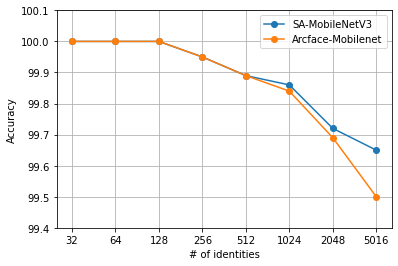
\includegraphics[width=0.5\textwidth]{image5-1}
  	\caption{دقت روش پیشنهادی در مقایسه با روش \lr{ArcFace}}
\end{figure}

\subsection{سرعت پاسخ‌دهی}
با توجه به اینکه هدف اصلی روش پیشنهادی، اجرا بر روی تلفن همراه هوشمند می‌باشد، علاوه بر ارزیابی دقت دسته بندی، از لحاظ پیچیدگی شبکه، تعداد پارامترها، سرعت پاسخ‌دهی و زمان اجرای عملیات پیشرو \LTRfootnote{Forward} نیز روش پیشنهادی را در مقایسه با سایر روش‌ها سنجیده‌ایم. در جدول \ref{table5-4} نتایج حاصل از محاسبه پیچیدگی شبکه و تعداد پارامترها را در معماری‌های مختلف بر روی مجموعه داده‌ ImageNet مشاهده می‌کنید.

\begin{table}[ht]
	\label{table5-4}
	\begin{center}
		\caption{پیچیدگی شبکه و تعداد پارامترهای معماری های مختلف بر روی مجموعه‌داده ImageNet}
		\resizebox{\textwidth}{!}
		{
			\begin{tabular}{|c|c|c|c|c|c|c|c|}
				\hline 
				
				Model & \lr{Accuracy (imageNet)} & \lr{Number of Parameters} & \lr{Accuracy density} & \lr{Madds}   
				\\
				\hline 
				\hline
				\lr{ResNet50} & \lr{83.0} & \lr{25 M} & \lr{3.32} & \lr{8220 M}
				\\
				\hline 
				\lr{MobileNetV2} & \lr{72.56} & \lr{3.5 M} & \lr{20.73} & \lr{627.69 M}
				\\
				\hline
				\lr{MobileNetV3} & \lr{75.2} & \lr{5.4 M} & \lr{13.92} & \lr{448.69 M}
				\\
				\hline
				\lr{SA-MobileNetV3} & \lr{79.8} & \lr{3.8 M} & \lr{21.06} & \lr{445.68 M}
				\\
				\hline
				
		\end{tabular}}
	\end{center} 
\end{table} 

\noindent
برای مقایسه زمان اجرای الگوریتم روش پیشنهادی با روش ArcFace آزمایش سرعت را بر روی دستگاه \lr{Raspberry Pi} اجرا کردیم. مشخصات سخت افزاری این دستگاه به شرچ زیر می‌باشد:

\begin{itemize}
	\item
	\lr{Model: Raspberry Pi 4 Model B}
	\item
	\lr{CPU: Broadcom BCM2711, Quad core Cortex-A72 (ARM v8) 64-bit SoC @ 1.5GHz}
	\item
	\lr{Memory: 4GB}
	\item
	\lr{Operating System: Raspberry Pi OS, Kernel version: 5.10}
\end{itemize}


نتایج ارزیابی را به دو صورت ارائه کردیم. در حالت اول فقط زمان اجرای یک بار عملیات پیشرو در شبکه تشخیص چهره را گزارش دادیم و در حالت دوم زمان اجرای کامل خط لوله را گزارش دادیم. یک خط لوله کامل به معنای ضبط فریم، پیش پردازش، یافتن چهره، تراز کردن چهره‌ و تشخیص چهره می‌باشد. در جدول \ref{table5-5} نتایج حاصل از محاسبه سرعت آمده است.

\begin{table}[ht]
	\label{table5-5}
	\begin{center}
		\caption{نتایج زمانی بر روی \lr{Raspberry Pi} به ازای هر فریم}
		\resizebox{\textwidth}{!}
		{
			\begin{tabular}{|c|c|c|}
				\hline 
				\lr{Model}
				& 
				 زمان اجرای کل خط لوله
				\lr{Detection + Alignment + Recognition}
				& 
				 فقط زمان اجرای شبکه
				\lr{recognition}   
				\\
				\hline 
				\hline
				\lr{SA-MobileNetV3} & \lr{6 fps} & \lr{25 fps}
				\\
				\hline 
				\lr{Arcface-Mobilenet} & \lr{5 fps} & \lr{20 fps}
				\\
				\hline				
		\end{tabular}}
	\end{center} 
\end{table}  

\noindent
با توجه به نتایجی که در جدول‌ها و شکل‌ها ارائه شد، متوجه می‌شویم که روش پیشنهادی ما از لحاظ دقت دسته بندی و سرعت پردازش نسبت به سایر روش‌های جدید در این زمینه بهتر عمل می‌نماید. ما محدودیت منابع تلفن همراه را در نظر گرفتیم و بر مبنای آن روشی ارائه دادیم که علاوه بر پیچیدگی کم و سرعت مناسب، دارای دقت دسته بندی بسیار بالایی باشد. معماری شبکه عصبی ارائه شده در این پژوهش، علاوه بر مسئله تشخیص چهره، می‌تواند در سایر مسائل و مجموعه داده‌های عمومی نیز کارامد باشد.
